\documentclass[11pt]{article}
\usepackage[utf8]{inputenc}
\usepackage[T1]{fontenc}
\usepackage{fixltx2e}
\usepackage{graphicx}
\usepackage{longtable}
\usepackage{float}
\usepackage{wrapfig}
\usepackage{rotating}
\usepackage[normalem]{ulem}
\usepackage{amsmath}
\usepackage{textcomp}
\usepackage{marvosym}
\usepackage{wasysym}
\usepackage{amssymb}
\usepackage[hidelinks]{hyperref}
\usepackage{listings}
\usepackage{xcolor}
\usepackage{amsthm}
\usepackage{subcaption}

\newcommand{\n}[0]{\\[\baselineskip]}


\author{140011146}
\title{Curry\TeX\ Studios Game Manual}

\begin{document}

\maketitle

\section{Introduction}
The game itself has explanatory tips that pop up which explain most concepts of the game and introduce new concepts slowly. However, this manual will also cover all concepts and mechanics in the game for players.

\section{Workers}
The workers in the company are shown on the right hand side of the screen. 
\begin{figure}[H]
\centering
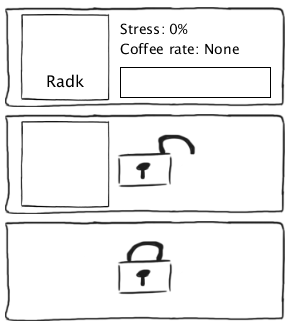
\includegraphics[width=0.4\textwidth, keepaspectratio]{imgs/all-workers.png}
\caption{Boxes on the right of the screen represent the workers in the company. The top box contains a worked named ``Radk", the middle box is unlocked, meaning a new worker can be recruited. The bottom box is locked and the player must buy upgrades to unlock this slot to allow a worker to be hired.}
\end{figure}
\noindent
The square boxes can be dragged to move the worker to different locations in the game to start an activity. The boxes also contain a bit of information about the worker. More detailed information can be viewed by \texttt{[Right-Clicking]} the worker box. 
\begin{figure}[H]
\centering
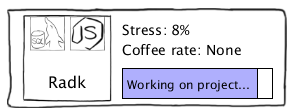
\includegraphics[width=0.6\textwidth, keepaspectratio]{imgs/worker.png}
\caption{A detailed look at a worker box, the square box represents the worker avatar, which contains the worker's name and the top two skills the worker has. Workers with two or less top skills will only have one or no icons here. The box also shows information about the worker's stress level, rate of coffee consumption and progress on any activity they are current doing.}
\end{figure}
\noindent
When workers work on a project, they will gain experience in the skills required for that project. Only the top two skills of a worker are displayed and active, but if a worker gains more experience in one skill, it will overtaking an existing one. Matching the appropriate skills to projects makes the worker more productive and faster for that project, and the worker will be slower if their skills don't match the project. 
\n
Workers with coffee addiction will want to drink coffee when working on projects. Drinking coffee will make them work a bit faster, but they will be slower if the company has run out of coffee. Additionally, if the company is out of coffee the worker may stall and stop working altogether until the more coffee arrives. To get coffee for the company, send a worker to the cafe.

\section{Locations}
There are many different locations that a worker's avatar box can be dragged to. Each location has a different activity for the worker to work on. For example, dragging the worker to the \texttt{[Restation]} lets them recover from stress. Workers with 100\% stress cannot do any activities except rest. To make workers work faster, the location can be clicked with the mouse and all workers currently working in that location will be sped up. Use this fact to put multiple workers on the same location and speed all of them up!

\subsection{Town locations}
The town locations are the locations in the center of the screen, the locations are buildings that the workers can be dragged to do different activities. 
\begin{figure}[H]
\centering
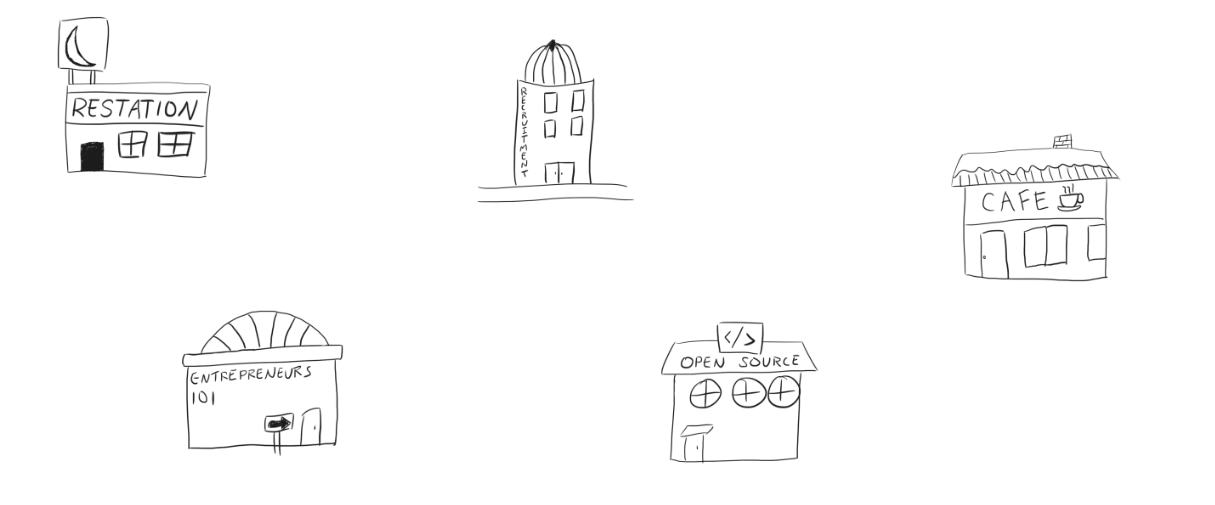
\includegraphics[width=0.8\textwidth, keepaspectratio]{imgs/town.png}
\caption{The town.}
\end{figure}
\noindent
Here are all the town locations and the activity they contain for a worker.
\begin{itemize}
\item The \texttt{[Restation]} allows a worker to recover from stress
\item \texttt{[Entrepreneurs 101]} allows a worker to increase their \texttt{[Entrepreneur]} stat, which gives them a chance to increase the money earned for a project each time they work on it.
\item \texttt{[Recruitment]} is the building to go to to recruit new workers. Workers can only be assigned there if there are free worker slots to hire new workers.
\item The \texttt{[Open Source]} building lets a worker increase their \texttt{[Fame]} stat, which gives them a chance to increase the reputation earned for a project each time they work on it.
\item The \texttt{[Cafe]} is the place to get coffee for the company.
\end{itemize}
\subsection{Project locations}
Below the town is the area of the office where workers get new projects and work on existing projects. 
\begin{figure}[H]
\centering
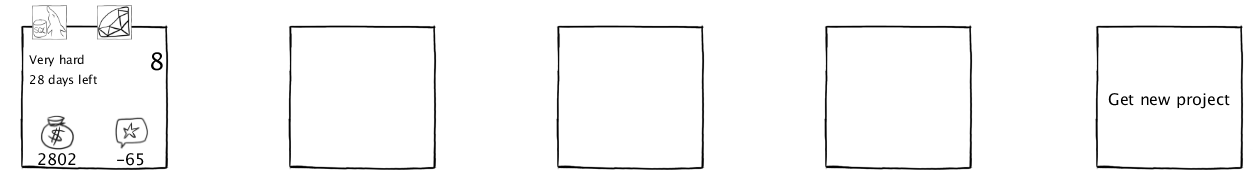
\includegraphics[width=1\textwidth, keepaspectratio]{imgs/office.png}
\end{figure}
\noindent
Workers can get new projects for the company by dragging them to the \texttt{[Get new project]} location. Workers can work on any existing project by dragging them to the corresponding project box. Each project box shows the skills required, difficulty, time limit, number of features and rewards for completing the project. Each time a worker works on a project, the number of features required to finish the project decreases by 1. 
\n
Some projects give more money and negative reputation while other projects give no money but lots of reputation. The player has to choose between how they want to balance and play the game and which aspect to focus on.

\section{Time}
The goal of the game is to get a certain number of reputation by 1 year. To get there, players should expand their company by buying upgrades and hiring more workers. 
\begin{figure}[H]
\centering
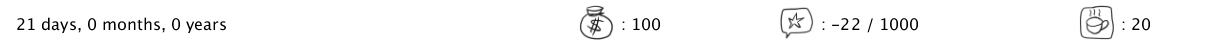
\includegraphics[width=1\textwidth, keepaspectratio]{imgs/topbar.png}
\caption{The top of the screen which shows the time, money, reputation and coffee.}
\end{figure}
\noindent
Time is very important because the player has to reach the reputation goal in 1 year. Time will continuously tick by while the player is in the main playing screen. Time will pause when the player is in a menu to give the player time to think and make decisions. Furthermore, every month, the company must pay salary to its workers. The company can go into debt paying salaries, but must be positive again before the start of the next month or the game is over!

\section{Money and reputation}
Money is important to pay salaries and buy upgrades and reputation is important to win the game. Additionally, more reputation increases the amount of money earned for projects according to the reputation for that project's skills. 
\begin{figure}[H]
\centering

\includegraphics[width=0.4\textwidth, keepaspectratio]{imgs/reputation.png}
\caption{Reputation analytics for each skill.}
\end{figure}
\noindent
The reputation for each skill is calculated differently compared to the total reputation. So a player might have high total reputation, but certain skills still have negative reputation. 

\end{document}